\documentclass[a4paper,12pt]{article} \usepackage{graphicx}
\usepackage{epstopdf} %\usepackage{gensymb} \usepackage{longtable}
\usepackage{graphicx}
%% Definitioner för LIPS-dokument

\usepackage[english,swedish]{babel}
\usepackage[utf8]{inputenc}
\usepackage[T1]{fontenc}
\usepackage{times}
\usepackage{ifthen}

\usepackage[margin=25mm]{geometry}

\usepackage{fancyhdr}
\pagestyle{fancy}
\lhead{}
\chead{\textbf{\LIPSprojekttitel}}
\rhead{\textbf{\textsl{LiTH}}\\\textbf{\LIPSdatum}}
\lfoot{\textbf{\LIPSkursnamn}\\\textbf{\LIPSdokumentansvarig}}
\cfoot{\textbf{\LIPSprojektgrupp}\\\textbf{\LIPSgruppepost}}
\rfoot{\textbf{\textsc{Lip}s}\\\textbf{Sida~\thepage}}

\setlength{\parindent}{0pt}
\setlength{\parskip}{1ex plus 0.5ex minus 0.2ex}


\newcommand{\twodigit}[1]{\ifthenelse{#1<10}{0}{}{#1}}
\newcommand{\dagensdatum}{\number\year-\twodigit{\number\month}-\twodigit{\number\day}}

%% ------------------------------------------
% NYBILD
% Skapar centrerad bild med caption
%   
% #1: Filens url relativt '/bilder/'
% #2:  Caption
% #3: Label
% #4: Skalning
%% ------------------------------------------
\newcommand{\nyBild}[4] 
{\begin{figure}[H]
  \centering
 \includegraphics[angle=0,scale=#4]{bilder/#1}
  \caption{#2}
  \label{fig:#3}
\end{figure}}



%%  Redefinitions of commands containing @
\makeatletter
\makeatother

\newcommand{\LIPStitelsida}{%
{\ }\vspace{45mm}
\begin{center}
  \textbf{\Huge \LIPSdokumenttyp}
\end{center}
\begin{center}
  {\Large Editor: \LIPSredaktor}
\end{center}
\begin{center}
  {\Large \textbf{Version \LIPSversion}}
\end{center}
\vfill
\begin{center}
  {\large Status}\\[1.5ex]
  \begin{tabular}{|*{3}{p{40mm}|}}
    \hline
    Reviewed & \LIPSgranskare & \LIPSgranskatdatum \\
    \hline
    Approved & \LIPSgodkannare & \LIPSgodkantdatum \\
    \hline
  \end{tabular}
\end{center}
\newpage
}


\newenvironment{LIPSprojektidentitet}{%
{\ }\vspace{45mm}
\begin{center}
  {\Large PROJECT IDENTITY}\\[0.5ex]
  {\small
  \LIPSartaltermin, \LIPSprojektgrupp\\
  Linköpings Tekniska Högskola, ISY
  }
\end{center}
\begin{center}
  {\small Group member}\\
%  \begin{tabular}{|p{30mm}|p{40mm}|p{35mm}|p{45mm}|}
  \begin{tabular}{|l|p{45mm}|p{25mm}|l|}
    \hline
    \textbf{Name} & \textbf{Responsibility} & \textbf{Phone} & \textbf{E-mail} \\
    \hline
}%
{%
    \hline
  \end{tabular}
\end{center}
\begin{center}
  {\small
    %\textbf{E-postlista för hela gruppen}: \LIPSgruppepost\\
    %\textbf{Hemsida}: \LIPSgrupphemsida\\[1ex]
    \textbf{Customer}: \LIPSkund\\
    \textbf{Customer Contact}: \LIPSkundkontakt\\
    \textbf{Course Leader}: \LIPSkursansvarig\\
    \textbf{Tutor}: \LIPShandledare\\
  }
\end{center}
\newpage
}
\newcommand{\LIPSgruppmedlem}[4]{\hline {#1} & {#2} & {#3} & {#4} \\}



\newenvironment{LIPSdokumenthistorik}{%
\begin{center}
  Document history\\[1ex]
  \begin{small}
    \begin{tabular}{|l|l|p{60mm}|l|l|}
      \hline
      \textbf{Version} & \textbf{Date} & \textbf{Changes} & \textbf{Edited by} & \textbf{Reviewed} \\
      }%
    {%
      \hline
    \end{tabular}
  \end{small}
\end{center}
}
\newcommand{\LIPSversionsinfo}[5]{\hline {#1} & {#2} & {#3} & {#4} & {#5} \\}

\newcounter{LIPSkravnummer}
\newcounter{LIPSunderkravnummer}[LIPSkravnummer]

\newenvironment{LIPSkravlista}{%
  \begin{tabular}{|p{25mm}|p{25mm}|p{85mm}|p{5mm}|}
    }%
  {%
    \hline
  \end{tabular}
}

\newenvironment{LIPSleveranslista}{%
  \begin{tabular}{|p{25mm}|p{20mm}|p{65mm}|p{25mm}|p{5mm}|}
    }%
  {%
    \hline
  \end{tabular}
}


\newcommand{\LIPSkrav}[3]
{\hline
\stepcounter{LIPSkravnummer}\textbf{Krav nr \arabic{LIPSkravnummer}} &
\textbf{{#1}} & 
{#2} & 
\textbf{{#3}} 
\\}

\newcommand{\LIPSleverans}[4]
{\hline
        \textbf{{#1}} & 
        {#2} & 
        {#3} & 
        \textbf {{#4}} 
\\}

\newcommand{\LIPSunderkrav}[3]{\hline\stepcounter{LIPSunderkravnummer}\textbf{Requirement nr \arabic{LIPSkravnummer}\Alph{LIPSunderkravnummer}} & \textbf{{#1}} & {#2} & \textbf{{#3}} \\}





%%% Local Variables: 
%%% mode: latex
%%% TeX-master: "kravspec_mall"
%%% End: 


\newcommand{\degree}{\ensuremath{^\circ}}
\newcommand{\LIPSartaltermin}{2013/VT}
\newcommand{\LIPSkursnamn}{TSEK06}
\newcommand{\LIPSprojekttitel}{DLL Based Frequency Multiplier}

\newcommand{\LIPSprojektgrupp}{Group 7}

\newcommand{\LIPSgruppepost}{}
\newcommand{\LIPSgrupphemsida}{} 
\newcommand{\LIPSdokumentansvarig}{Gustav Svensk}

\newcommand{\LIPSkund}{ISY, Linköpings universitet, 581\,83 Linköping}

\newcommand{\LIPSkundkontakt}{Amin Ojani}
\newcommand{\LIPSkursansvarig}{Atila Alvandpour}
\newcommand{\LIPShandledare}{Amin Ojani}



\newcommand{\LIPSdokumenttyp}{Project Plan} 
\newcommand{\LIPSredaktor}{Nora Björklund} 
\newcommand{\LIPSversion}{0.1} 
\newcommand{\LIPSdatum}{\dagensdatum}

\newcommand{\LIPSgranskare}{} 
\newcommand{\LIPSgranskatdatum}{}
\newcommand{\LIPSgodkannare}{} 
\newcommand{\LIPSgodkantdatum}{}


\begin{document}
\LIPStitelsida

%% Argument till \LIPSgruppmedlem: namn, roll i gruppen, telefonnummer, epost
\selectlanguage{swedish}
\begin{LIPSprojektidentitet}
 
\LIPSgruppmedlem{Nora Björklund}{Project leader}{076 7756
789}{norbj648@student.liu.se}
\LIPSgruppmedlem{\LIPSdokumentansvarig}{Documentation}{073
6208776}{grulfen3@gmail.com} 
\LIPSgruppmedlem{Christopher Hallberg}{}{0739845945}{chrha007@student.liu.se} 
\LIPSgruppmedlem{Gustaf Bengtz}{}{07073607307}{gbengtz@gmail.com} 
\LIPSgruppmedlem{Johan Berneland}{}{0704988329}{johbe915@student.liu.se}
\end{LIPSprojektidentitet}

\selectlanguage{english}

\tableofcontents{} 
\newpage %% Argument till \LIPSversionsinfo: versionsnummer, datum, ändringar,
         %  utfört av,granskat av
\addcontentsline{toc}{section}{Document history} \begin{LIPSdokumenthistorik} 
\LIPSversionsinfo{0.1}{}{First draft.}{}{}\end{LIPSdokumenthistorik} 
\newpage

\section{Customer}
The customer is Amin Ojani from the department of Electrical Engineering, Linköping University.

\section{Project Outline}
This project is the main part of the course TSEK06 - VLSI Chip Design Project.
The purpose of this project is to design a DLL-Based frequency multiplier.
DLL stands for delay-lock loop.

\subsection{Project Goal}
From \cite{project_spec} ``The project goal is to design an integrated circuit
(IC) in complementary metal-oxide
semiconductor (CMOS) technology. Students, participating in this project as
project members
and project leaders, should learn the different steps of the IC design flow.
That includes the
given system architecture analysis, simulation, layout implementation and
verification. The
project students have an optional choice to manufacture the designed IC circuit
on a chip. To
test the manufactured chips, another course (TSEK11) is available after the
project.''


\subsection{Deliverables}

\begin{LIPSleveranslista}
        \LIPSleverans{Delivery}{\textbf{Responsible}}{\textbf{Purpose}}
                     {Deadline}
        \LIPSleverans{High-level simulation result}{Nora Björklund}
                     {Simulation results from high-level, ensuring the functionality of the model}{11/2 -13}
        \LIPSleverans{Transistor-level simulation result}{Nora Björklund}{Simulation results from the gate/transistor level, ensuring the functionality of the design}{11/3 -13}
        \LIPSleverans{Completed chip}{Nora Björklund}{The final design files for the chip}{13/5 -13}
        \LIPSleverans{Final report}{Gustav Svensk}{Report indicating the functionality and how to use the chip}{24/5 -13}
\end{LIPSleveranslista}


\subsection{Limitations}
The final chip shall fulfill the requirements specified in section
\ref{sec:requirements}.
The requirements with priority level High will be focused on first and the other
requirements
will be focused on only after all the requirements with higher priority level
have been met.

\section{System Components}

The system consists of the following components.

\subsection{Phase Detector}
The Phase Detector (PD) is in charge of checking whether the input frequency 
and the produced frequency are in phase. The reference frequency is used as an 
input for a D flip-flop (DFF), while the produced frequency clock is used as 
the input of the DFF. If the produced signal is running late, it will not yet 
have risen when it should have, which means that the output from the DFF 
should be set low. Respectively, the output from the DFF will be high if the 
signal is running early. The output from the DFF will then be sent to the 
counter for further processing.

If the output from the PD starts toggling between low and high the phases of 
the clocks are as close to in phase as they can be. When this happens, the PD 
as well as the counter will be shut off to save energy. This will result in 
the reference and produced clocks to shift slightly and after a while they will 
not be in phase anymore. When this happens the PD and counter will be turned 
on again to get them into phase once more.

\subsection{Digital Counter}
The Digital Counter is used to determine how the delay line is supposed to 
adjust for the phase of the produced counter signal. It takes the output from 
the PD and if the output is high, it increments the internal value, while it 
decreases the internal value if the output from the PD is low. The input value 
is then used to determine how much the delay line should delay the signal. 

\subsection{Delay Line}

The delay line delays the signal in steps, the output between the steps will be
combined to produce the output signal of the system. The main components
of the delay line are an even number of inverters.  When the input signal has
passed through the entire delay line it will have been phase-shifted 360\degree. 
The delay of each stage will be set by binary-weighted capacitive loads
controlled by the output from the 6-bit binary counter. Preliminary  the
system will have 8 delay stages, each delaying the signal 45\degree. This makes
it possible to generate an output frequency 4 times that of the input. With this
it is also possible to choose signal components so that the output frequency is
2 times that of the input.

Depending on available space on the chip and available time the preliminary
number of 8 delay stages might be increased further. For example to a total of
16 stages giving 8 times the input frequency on the output. However, since space
is limited this improvement will hold low priority.

\subsection{Frequency Multiplier}
The frequency multiplier combines multiple phase-shifted versions of the input
signal to a higher frequency signal, essentially multiplying the frequency of
the input signal. This can be accomplished by letting the phase-shifted
signals be inputs to a multiplexer and the output of the multiplexer is the 
clock input to a counter. The output of the counter controls the multiplexer.
The frequency multiplied output is taken from the LSB of the counter output.

Preliminary the system will have 8 phase-shifted signals, 
each delayed 45\degree with respect to the previous signal.
Therefore a 3-bit counter is necessary. The LSB of the counter output will 
have a frequency that is 4 times the frequency of the input signal.
A block diagram of the frequency multiplier can be seen in 
figure \ref{fig:freq_mult}.

\begin{figure}[h!]
        \centering
        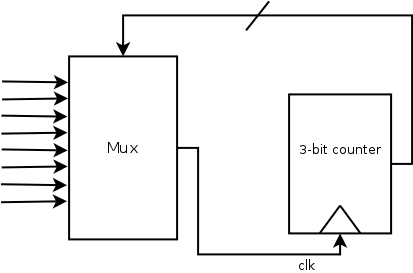
\includegraphics[width=0.5\textwidth]{../Bilder/freq_mult.png}
        \caption{Frequency multiplier}
        \label{fig:freq_mult}
\end{figure}

\section{Project Phases} 
This section briefly describes the outline of the different phases of the
project.
\subsection{Before Project}
Before starting with the high level design of the DLL the group will hold
preparatory meetings for planning the project and specify the written project
plan. The group members will also study up on relevant material concerning
functionality and implementation of a DLL.
  
\subsection{Under Project}
The project will start with implementing a high level model of the DLL using
the hardware definition language Verilog-A and running simulation on this
model. Thereafter the model will be implemented on gate/transistor level followed by
simulation. When the DLL behaves correctly on transistor level the work will
continue with the layout of the chip, DRC, parasitic extraction, LVS,
post-layout simulations, modification and chip evaluations. Finally the chip
layout will be sent to the foundry for fabrication.

\subsection{After Project}
When the chip layout has been sent to the foundry for fabrication a presentation
will be held where the stages of the project and results will be presented. 
Thereafter a more detailed final report will be written and submitted to the 
concerned parties. With this the project is considered finalized. In HT-13 there
is a course where the produced chip can be tested. The majority of the project
group members will take this course at this occasion.


\section{Organization Plan}
This section describes the organization of the project and the different
parties involved.

\subsection{Definition of parties and tasks}
\begin{enumerate}
        \item{Customer: Amin Ojani}
        \item{Project supervisor: Amin Ojani}

                Tasks:
                \begin{itemize}
                        \item{Formulate the project requirements}
                        \item{Provides technical support}
                        \item{Reviews the project documents}
                \end{itemize}
        \item{Project leader}

                Tasks:
                \begin{itemize}
                        \item{Responsible for organization of the team and the project planning}
                        \item{Divides the design and documentation work in an efficient way}
                        \item{Organizes the team meetings as well as the meetings between the team and supervisor}
                        \item{Keeps the supervisor informed about the progress of the project}
                \end{itemize}
        \item{Project design members (including the project leader)}

                Tasks:
                \begin{itemize}
                        \item{Are equally responsible for project planning and design}
                        \item{Participate actively in all the meetings}
                        \item{Support the team and the project leader}
                        \item{Keep the team and project leader informed about the progress of their tasks}
                \end{itemize}
\end{enumerate}

\subsection{Areas of respinsibility within the group}
The areas of responsibility is divided within the group in such a way that each
task has one person that is in charge of the task and one person that is his or
her dedicated helper. Each person in the group is in charge of one task and 
dedicated helper of another. Ther person in charge is responsible for planning 
and keeping track of the status of that task while the dedicated helper's 
responsibility is to help when possible/needed.

\begin{longtable}{|p{40mm}|p{50mm}|p{50mm}|}
        \hline
        \textbf{Task} & \textbf{In charge} & \textbf{Dedicated helper} \\
        \hline
        Phase Detector & GB & NB \\
        \hline
        Digital Counter & JB & GB \\
        \hline
        Delay Line  & CH & JB \\
        \hline
        Frequency Multiplier & GS & CH \\
        \hline
\end{longtable}



\section{Documentation Plan}
This section lists the documents that will be sent to the project supervisor.

\begin{longtable}{|p{40mm}|p{80mm}|p{30mm}|}
        \hline
        \textbf{Document} & \textbf{Description} & \textbf{Deadline} \\
        \hline
        Project plan & Describes the outline of the project & Week 5 \\
        \hline
        High-level modeling design and simulation result & Simulations results from high-level modeling & February 11 \\
        \hline
        Gate/Transistor level modeling design and simulation result  & Simulations results from gate/transistor level modeling & March 11 \\
        \hline
        Final Report & Description of the final product and experiences from the project & May 24 \\
        \hline
\end{longtable}


\section{Education}
This section specifies the education of group members and customer respectively.
\subsection{Project Group Education}
Each group member takes responsibility to study material relevant to both the
whole project and his or her designated tasks. 

\subsection{Customer Education}
The information needed for the customer to use the product will be included in
the final report.

\section{Meeting Plan}
The plan for the group is to hold one internal meeting each week as well as one meeting with the supervisor.
Additionally the group shall send one mail each week describing the progress of the project.

\section{Resource Plan} 
This section describes the available resources for the project.
\subsection{Persons} 
Supervisor - Amin Ojani
\subsection{Materiel}
\begin{itemize}
        \item{Scientific publication database}
        \item{IEL - IEEE/IEE Electronic Library, http://www.bibl.liu.se/english/databas/}
        \item{Circuit simulation and layout tool from Cadence$^{\textregistered}$, http://www.cadence.com/}
\end{itemize}

\subsection{Labs}
The project group will have access to the computer 
labs of the department of Electrical Engineering.


\section{Requirements}
\label{sec:requirements}
\begin{LIPSkravlista}
        \LIPSkrav{Design for low power}{Medium}
\LIPSkrav{Integrate as many system components as possible on-chip}{High}       
\LIPSkrav{Schematic and layout must be verified by simulation}{High}
\LIPSkrav{On-chip evaluation should be implemented, for full speed
testing}{High}
\LIPSkrav{Multiplied clock frequency at nominal supply (3.3V)>1 GHz}{High}
\LIPSkrav{Simulated chip power consumption < 100mW (3.3V supply)}{Medium}
\LIPSkrav{Simulated circuit power (normal activity) < 50mW (3.3V
supply)}{Medium}
        \LIPSkrav{Maximum transistor sizing = 20$\mu$m}{Medium}
        \LIPSkrav{Chip core area < 0.27mm$^2$}{High}
        \LIPSkrav{ Total project pin count: 12 }{High}
        \LIPSkrav{ Design technology is AMS 4-Metal 0.35 $\mu$m CMOS }{High}
\LIPSkrav{ The most important system nodes should have off-chip access pins
}{Medium}
        \LIPSkrav{ On-chip current densities < 1 mA/$\mu$m }{High}
        \LIPSkrav{ All requirements fulfilled in “typical”, “slow”, and “fast”
process Medium corners and for temperatures between 25 and 110 $^\circ$C }{High}\end{LIPSkravlista}

\section{Milestones and Deadlines}
This section lists the milestones and deadlines of the project.
The deadlines marked with \textbf{DEADLINE} are hard 
deadlines that can not be adjusted.

\begin{LIPSdeadlines}
        \LIPSdeadline{Project selection}{January 18}
        \LIPSdeadline{High-level modeling design and simulation result (report)}{February 11}
        \LIPSdeadline{Gate/Transistor level design and simulation result (report)}{March 11}
        \LIPSdeadline{Layout, DRC, parasitic extraction, LVS, post-layout simulations, modification and chip evaluations}{May 6}
        \LIPSdeadline{\textbf{DEADLINE}, Delivery of the completed chip}{May 13}
        \LIPSdeadline{\textbf{DEADLINE}, Final report and oral presentation}{May 24}
\end{LIPSdeadlines}

\section{Time plan}
The time plan is a separate document.

\section{Quality Plan} 
The quality plan below is what the group plans to do to ensure functionality of the chip. 
\subsection{Simulations} 
The following should be verified by simulations,

\begin{itemize}
\item High-level design
\item Schematic
\item Layout
\item Chip power consumption
\item Chip circuit power
\end{itemize}

\newpage 
\appendix 
\newpage


\addcontentsline{toc}{section}{References}
\begin{thebibliography}{99}
\bibitem{project_spec}\textit{Project: DLL-Based Frequency Multiplier - } Bhide,
Ameya
\\ http://www.ek.isy.liu.se/courses/tsek06/ 2013-01-27

\bibitem{dll_clock}\textit{A Low-Power Digital DLL-Based Clock Generator in Open-Loop Mode - }
Behzad Mesgarzadeh, Atila Alvandpour \\
IEEE Journal of Solid-State Circuits. Vol. 44. No. 7. July 2009

\end{thebibliography}


\end{document} 

%%% Local Variables: %%% mode: latex %%% TeX-master: t %%% End:
